Bulk Method is a design pattern that allows the user to call a method on a collection of objects.
There are usually pairs of methods, one that operates on a single object and one that operates
on a collection of objects.
It is possible to consider this design pattern to be a specific subtype of the Method Multiplication approach.

Following Figure~\ref{fig:bulk_write_packets} shows application of the Bulk Method design pattern to the
API method for writing a collection of IGMP Query Membership packets.
There are small adjustments in comparison to version of the method that writes a single packet:

\begin{itemize}
    \item The method name is \textit{writeQueryMembershipPackets} to better reflect its functionality.
    \item The method accepts a collection of group addresses that are queried by the IGMP Query Membership packets.
    \item The method accepts collection of \textit{NetInterface} objects instead of a single \textit{OutputStream}
    stream that is bound to a single network interface.
    The idea is to leverage advantages of the Bulk Method design pattern and load-balance the work between multiple
    output network interfaces.
\end{itemize}

\begin{figure}[!htb]
    \centering
    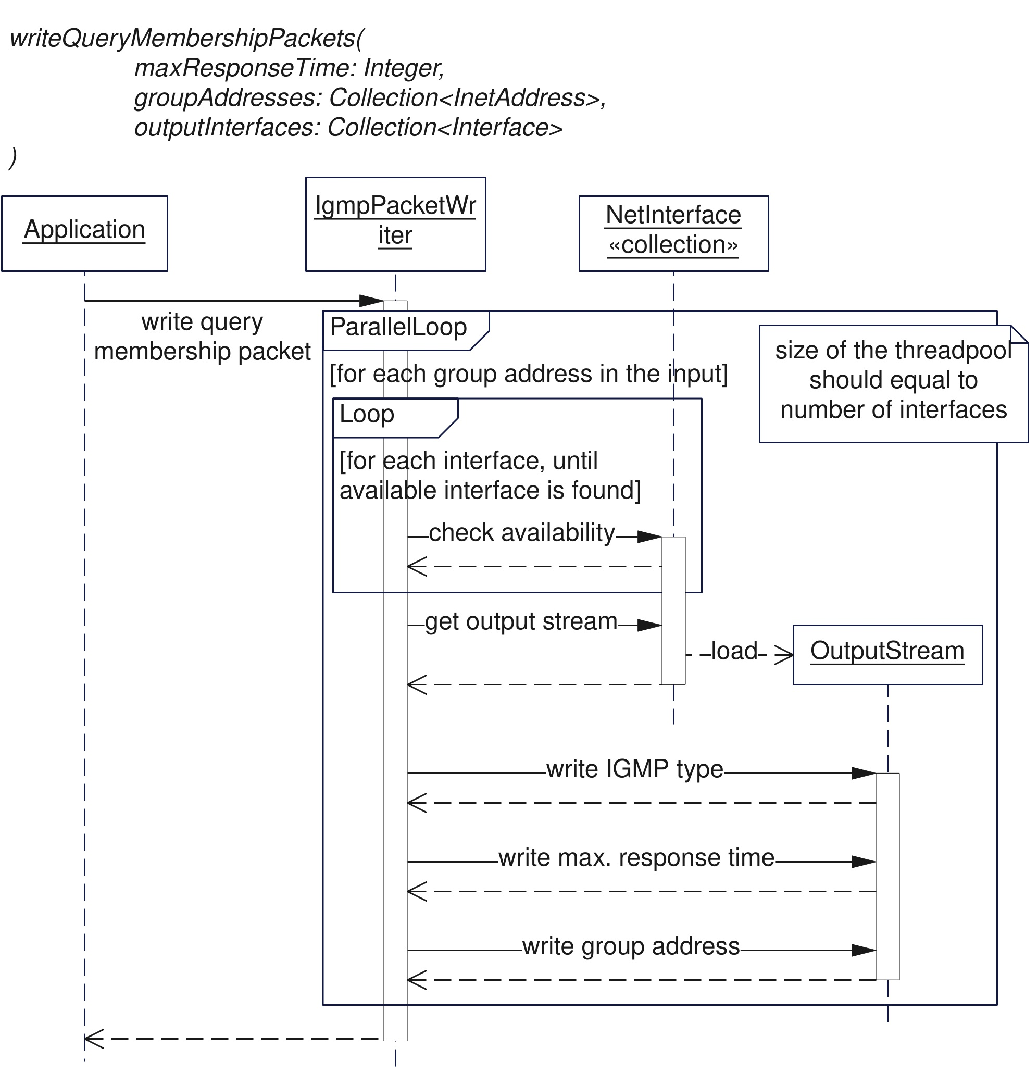
\includegraphics[width=1.0
    \textwidth]{bulk_write_packets}
    \caption{Bulk Method: Writing collection of IGMP Query Membership packets}
    \label{fig:bulk_write_packets}
\end{figure}

Benefits of the Bulk Method design pattern:

\begin{itemize}
    \item Efficiency - The implementation may optimize the work by processing the collection of objects
    in a single pass instead of processing each object individually.
    For example, the single transaction and single lock acquisition may be used to process multiple objects.
    The implementation may also be able to process multiple objects in parallel.
    \item Simplicity - From the client's perspective, the Bulk Method design pattern is simpler to use than
    performing the same operation on each object individually in the loop on the client side.
\end{itemize}

Drawbacks of the Bulk Method design pattern:

\begin{itemize}
    \item Lack of flexibility - There could be multiple versions of the Bulk Method implemented based on
    various requirements from different clients.
    For example, one client may require the Bulk Method to be atomic, while another client may not.
    It is usually not possible to satisfy all requirements with a single version of the Bulk Method.
    Because of this, the Bulk Method design pattern may lead to code duplication and decreased maintainability of code.
    \item Artificial creation of useless Bulk Methods - It could be tempting to create a Bulk Method for each
    method that operates on a single object.
    However, this is not a good idea because of the increased maintenance cost, increased code complexity,
    and finally missing use-cases.
    The Bulk Method design pattern should be used only when there is a real use-case for it, and it is possible
    to implement it more efficiently than the client would do by simple looping over the collection of objects.
\end{itemize}

Common use-cases of the Bulk Method design pattern:

\begin{itemize}
    \item It is possible to process multiple objects in a single transaction that assures Atomicity, Consistency,
    Isolation, and Durability (ACID) properties.
    \item Processing multiple objects in a parallel fashion.
\end{itemize}
